\documentclass[9pt,portrait]{article}
\usepackage{beamerarticle} % makes slides into article

%% xcolor Option Clash issue
%	Do not include xcolor,, tikz-qtree, todonotes, here do it after beamerarticle
\usepackage{multicol}
\usepackage{booktabs}
\usepackage{calc}
\usepackage{ifthen}
\usepackage[portrait]{geometry}
\usepackage{hyperref}
\usepackage{color}
\usepackage{enumitem}
\usepackage{textcomp} 				% copyleft symbol
\usepackage{verbatim}
\usepackage{adjustbox} 				% for resizebox to adjust table figure content
\usepackage{enumitem}				% margin free lists
\usepackage{amsmath}
\usepackage{mathrsfs}
\usepackage{csvsimple}				% importing csv as table
\usepackage{textcomp} 				% copyleft symbol
\usepackage{graphicx}
\usepackage{etoolbox} % conditional inclusions

\usepackage{media9}
 \usepackage{multimedia}
 \usepackage{makecell}
 \usepackage{listings}
%  \usepackage{color}
 
\definecolor{codegreen}{rgb}{0,0.6,0}
\definecolor{codegray}{rgb}{0.5,0.5,0.5}
\definecolor{codepurple}{rgb}{0.58,0,0.82}
\definecolor{backcolour}{rgb}{.914, .89, .957} % pale purple

\definecolor{mygreen}{rgb}{0,0.6,0}
\definecolor{mygray}{rgb}{0.5,0.5,0.5}
\definecolor{mymauve}{rgb}{0.58,0,0.82}

\lstdefinestyle{mystyle}{
  backgroundcolor=\color{backcolour},   % choose the background color; you must add \usepackage{color} or \usepackage{xcolor}; should come as last argument
  basicstyle=\footnotesize\ttfamily,       % the size of the fonts that are used for the code
  breakatwhitespace=true,          % sets if automatic breaks should only happen at whitespace
  breaklines=true,                 % sets automatic line breaking
  captionpos=b,                    % sets the caption-position to bottom
  commentstyle=\color{mygreen},    % comment style
  deletekeywords={...},            % if you want to delete keywords from the given language
  escapeinside={\%*}{*)},          % if you want to add LaTeX within your code
  extendedchars=true,              % lets you use non-ASCII characters; for 8-bits encodings only, does not work with UTF-8
  frame=single,	                   % adds a frame around the code
  keepspaces=true,                 % keeps spaces in text, useful for keeping indentation of code (possibly needs columns=flexible)
  keywordstyle=\color{blue},       % keyword style
  language=Python,                 % the language of the code
  morekeywords={*,...},            % if you want to add more keywords to the set
  % numbers=left,                    % where to put the line-numbers; possible values are (none, left, right)
  % numbersep=5pt,                   % how far the line-numbers are from the code
  % numberstyle=\tiny\color{mygray}, % the style that is used for the line-numbers
  rulecolor=\color{black},         % if not set, the frame-color may be changed on line-breaks within not-black text (e.g. comments (green here))
  showspaces=false,                % show spaces everywhere adding particular underscores; it overrides 'showstringspaces'
  showstringspaces=false,          % underline spaces within strings only
  showtabs=false,                  % show tabs within strings adding particular underscores
  stepnumber=2,                    % the step between two line-numbers. If it's 1, each line will be numbered
  stringstyle=\color{codepurple},  % string literal style
  tabsize=2,	                   % sets default tabsize to 2 spaces
  columns=fullflexible,
  linewidth=0.98\linewidth,        % Box width
  aboveskip=10pt,	   			   % Space before listing 
  belowskip=-15pt,	   			   % Space after listing  
  xleftmargin=.02\linewidth,  
  title=\lstname                   % show the filename of files included with \lstinputlisting; also try caption instead of title
}


% \definecolor{codegreen}{rgb}{0,0.6,0}
% \definecolor{codegray}{rgb}{0.5,0.5,0.5}
% \definecolor{codepurple}{rgb}{0.58,0,0.82}
% %\definecolor{backcolour}{rgb}{0.95,0.95,0.92} % faint postman color
% \definecolor{backcolour}{rgb}{.914, .89, .957} % pale purple
% %\lstset{basicstyle=\footnotesize\ttfamily}

% \lstdefinestyle{mystyle}{
    % backgroundcolor=\color{backcolour},   
    % commentstyle=\color{codegreen},
    % keywordstyle=\color{magenta},
    % numberstyle=\tiny\color{codegray},
    % stringstyle=\color{codepurple},
    % basicstyle= \tiny\ttfamily %\scriptsize\ttfamily, %\footnotesize,  % the size of the fonts that are used for the code
    % breakatwhitespace=true,  % sets if automatic breaks should only happen at whitespace        
    % breaklines=true, % sets automatic line breaking   
    % linewidth=\linewidth,	
    % captionpos=b,                    
    % keepspaces=true,% keeps spaces in text, useful for keeping indentation                
% %    numbers=left,                  
    % numbers=none,  
% %    numbersep=5pt,                  
    % showspaces=false,                
    % showstringspaces=false,
    % showtabs=false,                  
    % tabsize=2
% }
\lstset{style=mystyle}


%\lstset{basicstyle=\footnotesize\ttfamily}

\newtoggle{VideoFrames}
\togglefalse{VideoFrames}


\newtoggle{CopyrightPictures}
\togglefalse{CopyrightPictures}

\hypersetup{ % remove ugly hyperlink boxes
    colorlinks,
    linkcolor={red!50!black},
    citecolor={blue!50!black}%,
    %urlcolor={green!80!black}
}

% This sets page margins to .5 inch if using letter paper, and to 1cm
% if using A4 paper. (This probably isn't strictly necessary.)
% If using another size paper, use default 1cm margins.
\ifthenelse{\lengthtest { \paperwidth = 8.5in}}
	{ \geometry{top=.2in,left=.25in,right=.25in,bottom=.5in} }
	{\ifthenelse{ \lengthtest{ \paperwidth = 290mm}}
		{\geometry{top=1cm,left=1cm,right=1cm,bottom=2cm} }
		{\geometry{top=1cm,left=1cm,right=1cm,bottom=2cm} }
	}

% % Turn off header and footer
% \pagestyle{empty}

\usepackage{fancyhdr}   % Package to customize headers and footers
% Turn ON header and footer
\pagestyle{fancy}

% Add a line above the footer
\renewcommand{\footrulewidth}{0.4pt}  % Set the line thickness (adjust as needed)
% Set footer content
\fancyfoot[C]{\textit{Yogesh Haribhau Kulkarni}} % Centered footer text
\fancyfoot[R]{\thepage}                       % Page number on the right
\fancyfoot[L]{\textit{\href{http://www.yogeshkulkarni.com}{yogeshkulkarni@yahoo.com}}} % Centered footer text

% Optional: Set header if needed
%\fancyhead[L]{\textit{Your Header Text Here}} % Header text on the left
 

% Redefine section commands to use less space
\makeatletter
\renewcommand{\section}{\@startsection{section}{1}{0mm}%
                                {-1ex plus -.5ex minus -.2ex}%
                                {0.5ex plus .2ex}%x
                                {\normalfont\large\bfseries}}
\renewcommand{\subsection}{\@startsection{subsection}{2}{0mm}%
                                {-1explus -.5ex minus -.2ex}%
                                {0.5ex plus .2ex}%
                                {\normalfont\normalsize\bfseries}}
\renewcommand{\subsubsection}{\@startsection{subsubsection}{3}{0mm}%
                                {-1ex plus -.5ex minus -.2ex}%
                                {1ex plus .2ex}%
                                {\normalfont\small\bfseries}}
\makeatother

% Define BibTeX command
\def\BibTeX{{\rm B\kern-.05em{\sc i\kern-.025em b}\kern-.08em
    T\kern-.1667em\lower.7ex\hbox{E}\kern-.125emX}}

% Don't print section numbers
\setcounter{secnumdepth}{0}

\newcommand{\code}[1]{\par\vskip0pt plus 1filll \footnotesize Code:~\itshape#1}


\setlength{\parindent}{0pt}
\setlength{\parskip}{0pt plus 0.5ex}
\setlength\columnsep{30pt}

\usepackage{tcolorbox}  % For creating fancy boxes
\usepackage{tikz}       % For drawing borders

% Define a fancy style for cover pages
\tcbuselibrary{skins, breakable, theorems}
\tcbset{
    coverstyle/.style={
        enhanced,
        colframe=black,
        colback=white,
        coltitle=black,
        fonttitle=\bfseries\LARGE,
        fontupper=\normalsize,
        boxrule=1mm,
        width=\textwidth,
        arc=4mm,
        boxsep=5mm,
        outer arc=0mm,
        attach boxed title to top center={yshift=-0.5cm},
        boxed title style={colframe=black, colback=white, boxrule=0mm},
    }
}
\usepackage{polyglossia}
\setdefaultlanguage{sanskrit}
\setotherlanguage{english}

\usepackage{fontspec}
\setmainfont{Segoe UI}
\newfontfamily\devanagarifont[Scale=MatchUppercase]{Nakula}
\newfontfamily\devtransl[Mapping=DevRom]{Segoe UI}

% Sharada Fonts
\newfontfamily\sharadafont[Script=Sharada]{Noto Sans Sharada}

\graphicspath{{images/}}


\begin{document}
\footnotesize


\begin{center}
\Large{\textbf{Introduction to Sharada Script\\ Yogesh Haribhau Kulkarni}}  
\end{center}

\begin{multicols}{2}
\section[Intro]{Introduction}
%%%%%%%%%%%%%%%%%%%%%%%%%%%%%%%%%%%%%%%%%%%%%%%%%%%%%%%%%%%%%%%%%%%%%%%%%%%%%%%%%%
\begin{frame}[fragile]\frametitle{}
\begin{center}
{\Large Introduction}
\end{center}
\end{frame}


%%%%%%%%%%%%%%%%%%%%%%%%%%%%%%%%%%%%%%%%%%%%%%%%%%%%%%%%%%%
\begin{frame}[fragile]\frametitle{Prayer}

{\sharadafont 𑆤𑆩𑆯𑇀𑆯𑆳𑆫𑆢𑆳𑆪𑆽 𑆤𑆩𑆱𑇀𑆠𑆼 𑆯𑆳𑆫𑆢𑆼 𑆢𑆼𑆮𑆴 𑆑𑆳𑆯𑇀𑆩𑆵𑆫𑆥𑆶𑆫𑆮𑆳𑆱𑆴𑆤𑆴 𑇅 𑆠𑇀𑆮𑆳𑆩𑆲𑆁 𑆥𑇀𑆫𑆳𑆫𑇀𑆡𑆪𑆼 𑆤𑆴𑆠𑇀𑆪𑆁 𑆮𑆴𑆢𑇀𑆪𑆳𑆢𑆳𑆤𑆁 𑆖 𑆢𑆼𑆲𑆴 𑆩𑆼 𑇆}

नमस्ते शारदे देवि काश्मीरपुरवासिनि । त्वामहं प्रार्थये नित्यं विद्यादानं च देहि मे ॥

namaste śārade devi kāśmīrapuravāsini . tvāmahaṃ prārthaye nityaṃ vidyādānaṃ ca dehi me ..

\end{frame}

%%%%%%%%%%%%%%%%%%%%%%%%%%%%%%%%%%%%%%%%%%%%%%%%%%%%%%%%%%%
\begin{frame}[fragile]\frametitle{Sarada Script}

\begin{itemize}
    \item Sarada script is a writing system used for the Kashmiri language by the educated Hindu minority in Kashmir and surrounding valleys.
    \item It is taught in Hindu schools but is not used in printing books.
    \item Originating in the 8th century AD, Sarada descended from the Gupta script of North India.
    \item Devanāgarī also developed from the Gupta script.
    \item The earliest inscriptions in Sarada script, found in Kashmir and northeastern Punjab, are dated AD 804.
    \item Sarada script corresponds letter for letter with Devanāgarī but differs greatly in shape with stiff, thick strokes.
    \item Muslims in Kashmir use a Persian-Arabic script.
    \item Much Kashmiri literature is written in Sanskrit using Devanāgarī script.
\end{itemize}

\end{frame}

%%%%%%%%%%%%%%%%%%%%%%%%%%%%%%%%%%%%%%%%%%%%%%%%%%%%%%%%%%%
\begin{frame}[fragile]\frametitle{Vowels}

	\begin{center}
	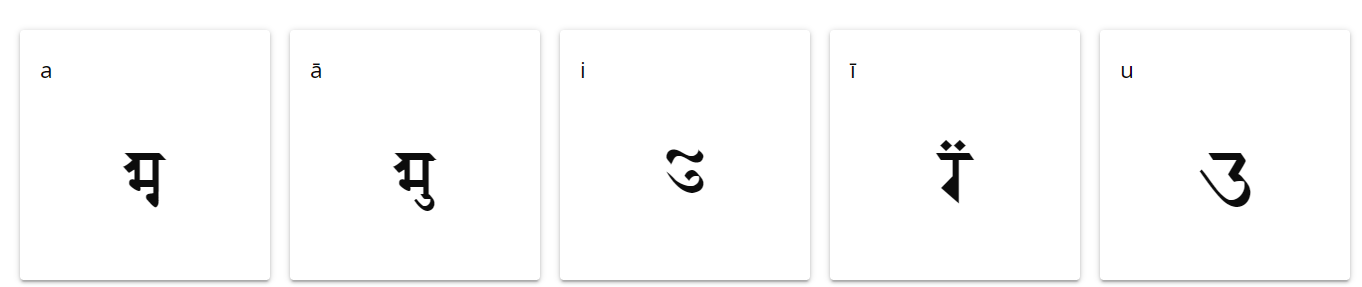
\includegraphics[width=\linewidth,keepaspectratio]{sharada_vowels_1} 
	
	{\tiny (Ref: Aksharamukha : Script Converter)}
	\end{center}	

\end{frame}

%%%%%%%%%%%%%%%%%%%%%%%%%%%%%%%%%%%%%%%%%%%%%%%%%%%%%%%%%%%
\begin{frame}[fragile]\frametitle{Vowels}

	\begin{center}
	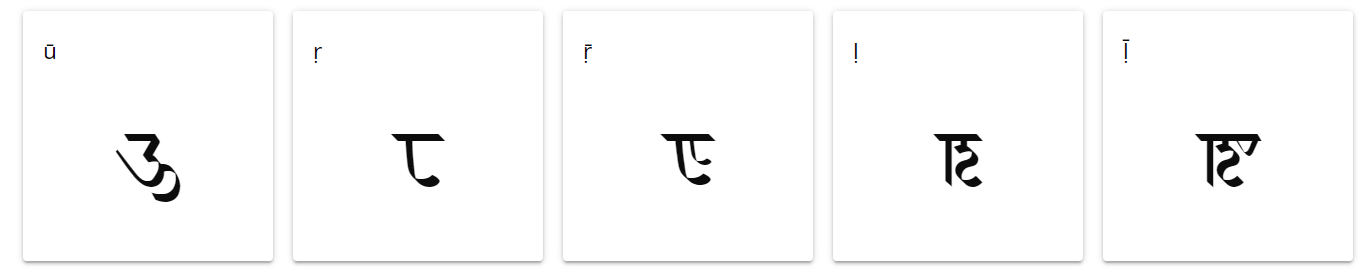
\includegraphics[width=\linewidth,keepaspectratio]{sharada_vowels_2} 
	
	{\tiny (Ref: Aksharamukha : Script Converter)}
	\end{center}	

\end{frame}

%%%%%%%%%%%%%%%%%%%%%%%%%%%%%%%%%%%%%%%%%%%%%%%%%%%%%%%%%%%
\begin{frame}[fragile]\frametitle{Vowels}

	\begin{center}
	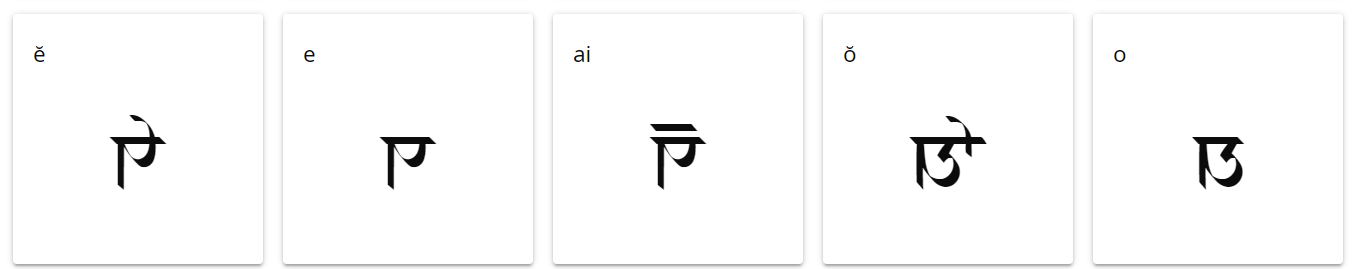
\includegraphics[width=\linewidth,keepaspectratio]{sharada_vowels_3} 
	
	{\tiny (Ref: Aksharamukha : Script Converter)}
	\end{center}	

\end{frame}

%%%%%%%%%%%%%%%%%%%%%%%%%%%%%%%%%%%%%%%%%%%%%%%%%%%%%%%%%%%
\begin{frame}[fragile]\frametitle{Vowels}

	\begin{center}
	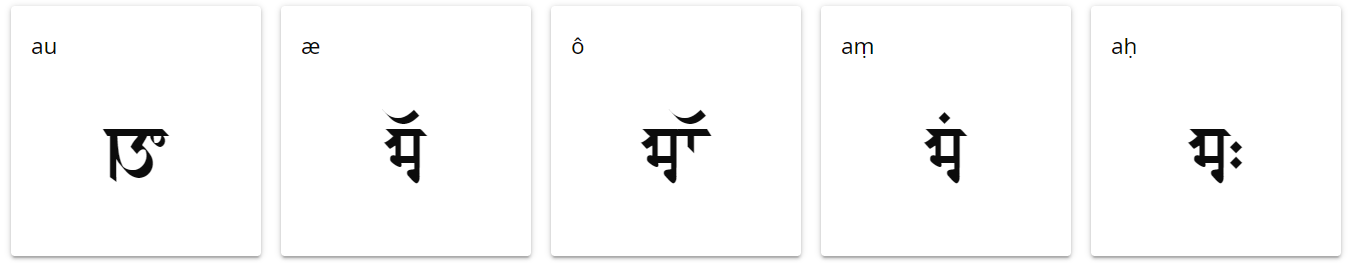
\includegraphics[width=\linewidth,keepaspectratio]{sharada_vowels_4} 
	
	{\tiny (Ref: Aksharamukha : Script Converter)}
	\end{center}	

\end{frame}

%%%%%%%%%%%%%%%%%%%%%%%%%%%%%%%%%%%%%%%%%%%%%%%%%%%%%%%%%%%
\begin{frame}[fragile]\frametitle{Vowels}

	\begin{center}
	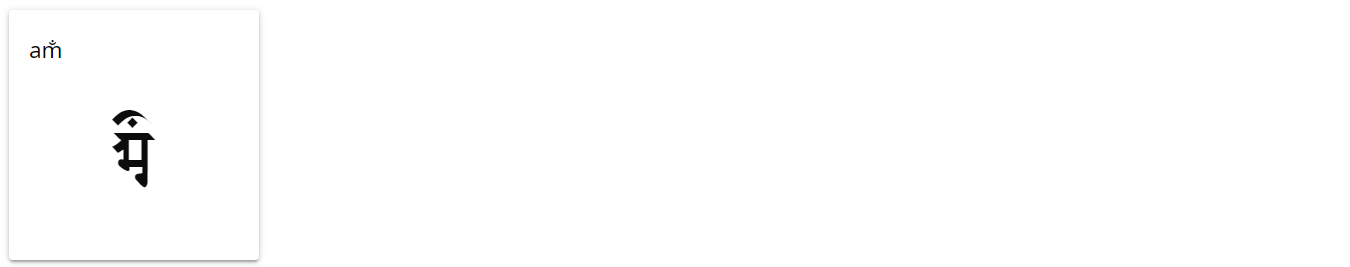
\includegraphics[width=\linewidth,keepaspectratio]{sharada_vowels_5} 
	
	{\tiny (Ref: Aksharamukha : Script Converter)}
	\end{center}	

\end{frame}

%%%%%%%%%%%%%%%%%%%%%%%%%%%%%%%%%%%%%%%%%%%%%%%%%%%%%%%%%%%
\begin{frame}[fragile]\frametitle{Consonants}

	\begin{center}
	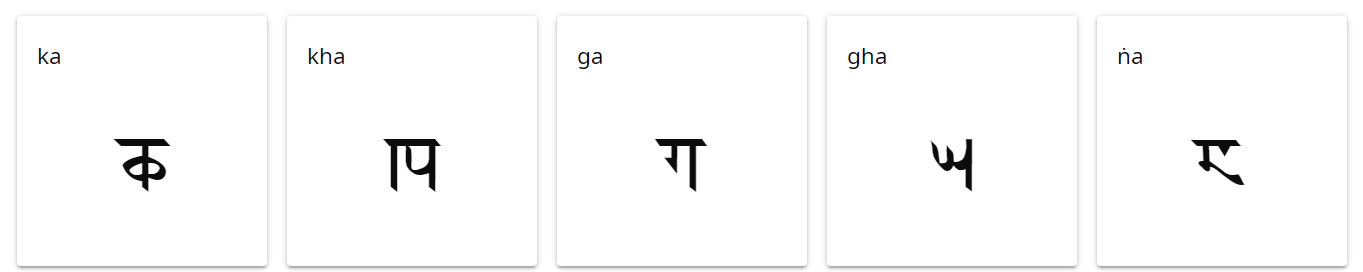
\includegraphics[width=\linewidth,keepaspectratio]{sharada_consonants_ka} 
	
	{\tiny (Ref: Aksharamukha : Script Converter)}
	\end{center}	

\end{frame}

%%%%%%%%%%%%%%%%%%%%%%%%%%%%%%%%%%%%%%%%%%%%%%%%%%%%%%%%%%%
\begin{frame}[fragile]\frametitle{Consonants}

	\begin{center}
	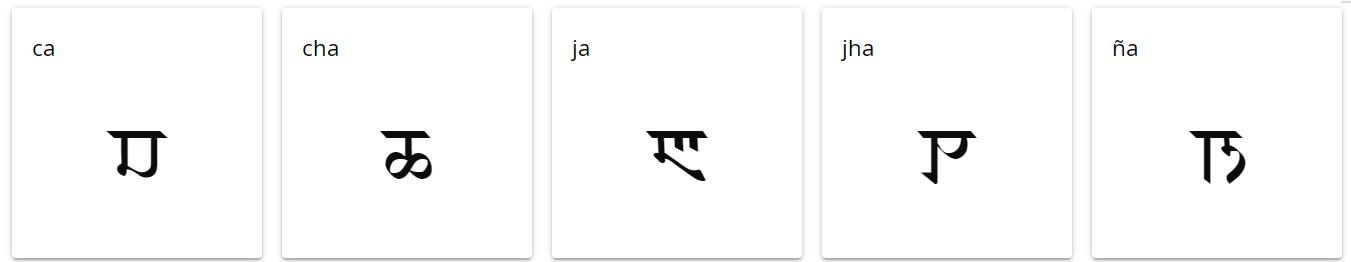
\includegraphics[width=\linewidth,keepaspectratio]{sharada_consonants_cha} 
	
	{\tiny (Ref: Aksharamukha : Script Converter)}
	\end{center}	

\end{frame}

%%%%%%%%%%%%%%%%%%%%%%%%%%%%%%%%%%%%%%%%%%%%%%%%%%%%%%%%%%%
\begin{frame}[fragile]\frametitle{Consonants}

	\begin{center}
	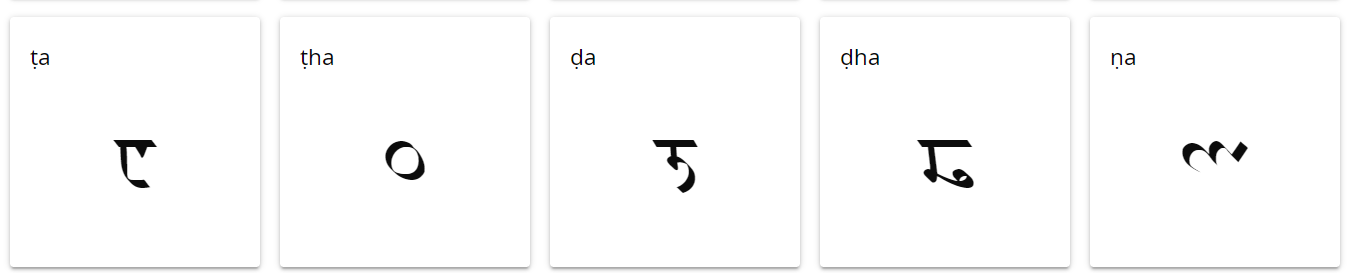
\includegraphics[width=\linewidth,keepaspectratio]{sharada_consonants_Ta} 
	
	{\tiny (Ref: Aksharamukha : Script Converter)}
	\end{center}	

\end{frame}

%%%%%%%%%%%%%%%%%%%%%%%%%%%%%%%%%%%%%%%%%%%%%%%%%%%%%%%%%%%
\begin{frame}[fragile]\frametitle{Consonants}

	\begin{center}
	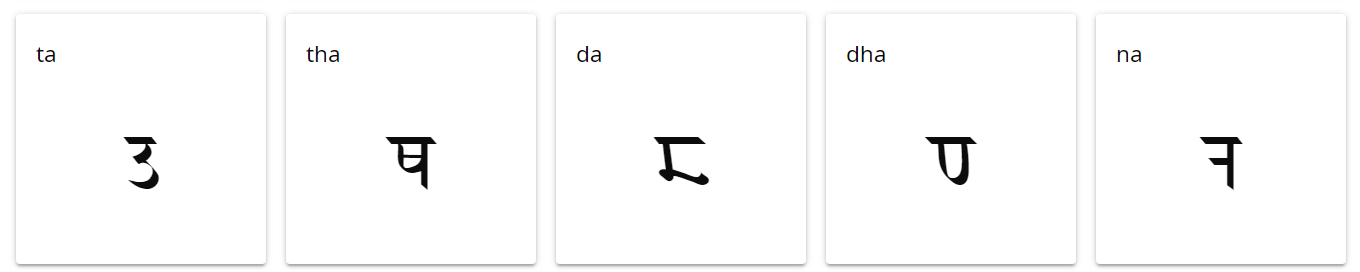
\includegraphics[width=\linewidth,keepaspectratio]{sharada_consonants_taa} 
	
	{\tiny (Ref: Aksharamukha : Script Converter)}
	\end{center}	

\end{frame}

%%%%%%%%%%%%%%%%%%%%%%%%%%%%%%%%%%%%%%%%%%%%%%%%%%%%%%%%%%%
\begin{frame}[fragile]\frametitle{Consonants}

	\begin{center}
	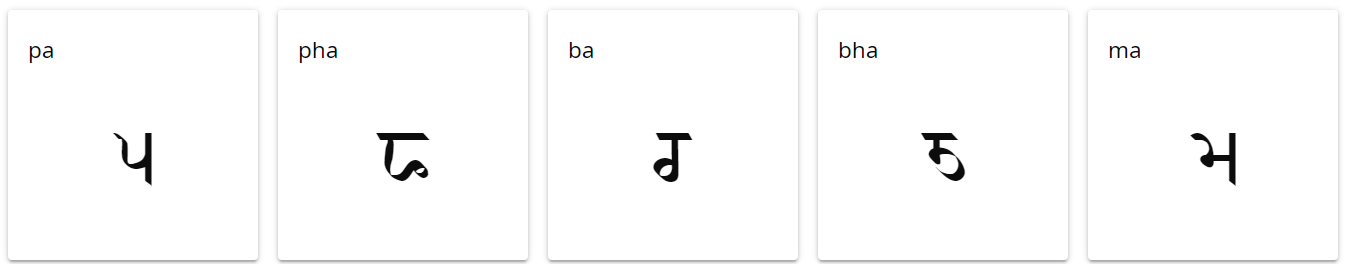
\includegraphics[width=\linewidth,keepaspectratio]{sharada_consonants_pa} 
	
	{\tiny (Ref: Aksharamukha : Script Converter)}
	\end{center}	

\end{frame}

%%%%%%%%%%%%%%%%%%%%%%%%%%%%%%%%%%%%%%%%%%%%%%%%%%%%%%%%%%%
\begin{frame}[fragile]\frametitle{Consonants}

	\begin{center}
	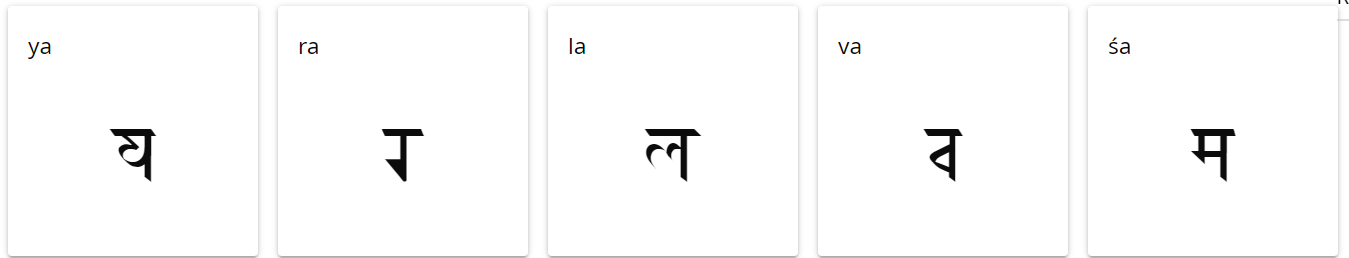
\includegraphics[width=\linewidth,keepaspectratio]{sharada_consonants_ya} 
	
	{\tiny (Ref: Aksharamukha : Script Converter)}
	\end{center}	

\end{frame}

%%%%%%%%%%%%%%%%%%%%%%%%%%%%%%%%%%%%%%%%%%%%%%%%%%%%%%%%%%%
\begin{frame}[fragile]\frametitle{Consonants}

	\begin{center}
	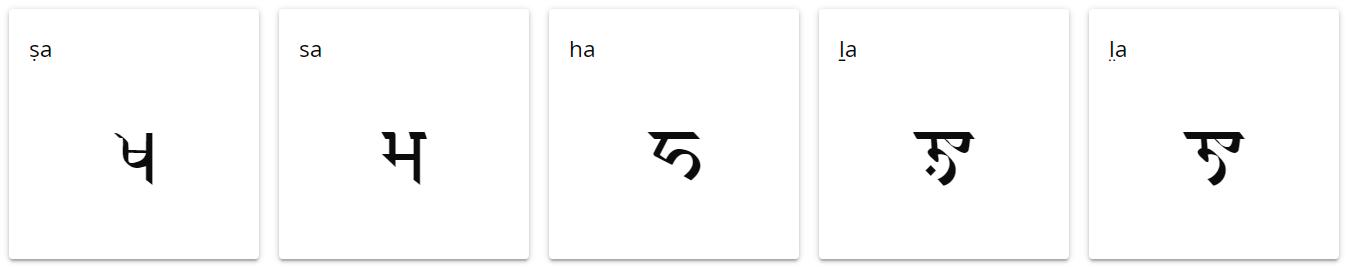
\includegraphics[width=\linewidth,keepaspectratio]{sharada_consonants_sha} 
	
	{\tiny (Ref: Aksharamukha : Script Converter)}
	\end{center}	

\end{frame}

%%%%%%%%%%%%%%%%%%%%%%%%%%%%%%%%%%%%%%%%%%%%%%%%%%%%%%%%%%%
\begin{frame}[fragile]\frametitle{Consonants}

	\begin{center}
	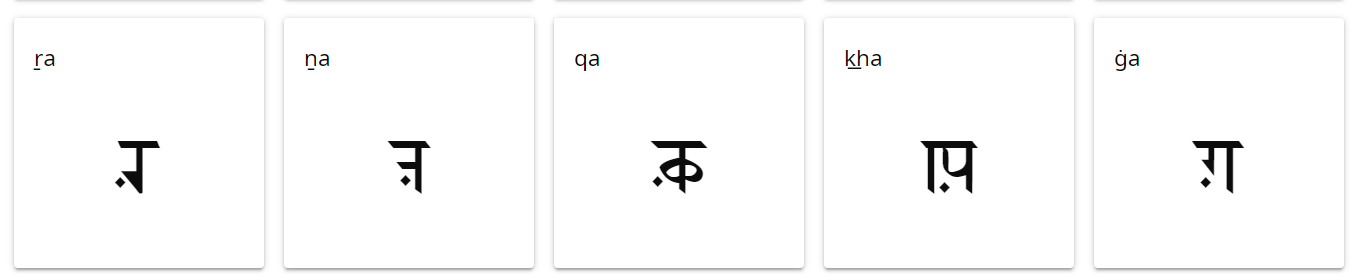
\includegraphics[width=\linewidth,keepaspectratio]{sharada_consonants_ra} 
	
	{\tiny (Ref: Aksharamukha : Script Converter)}
	\end{center}	

\end{frame}

%%%%%%%%%%%%%%%%%%%%%%%%%%%%%%%%%%%%%%%%%%%%%%%%%%%%%%%%%%%
\begin{frame}[fragile]\frametitle{Consonants}

	\begin{center}
	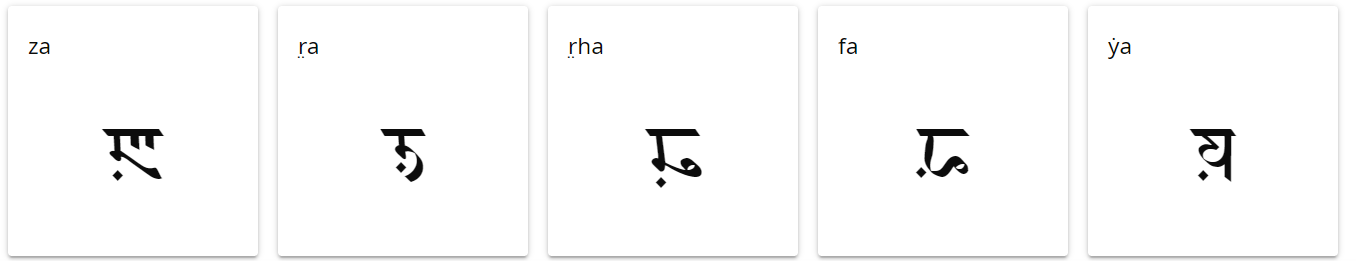
\includegraphics[width=\linewidth,keepaspectratio]{sharada_consonants_za} 
	
	{\tiny (Ref: Aksharamukha : Script Converter)}
	\end{center}	

\end{frame}

%%%%%%%%%%%%%%%%%%%%%%%%%%%%%%%%%%%%%%%%%%%%%%%%%%%%%%%%%%%
\begin{frame}[fragile]\frametitle{Compounds}

	\begin{center}
	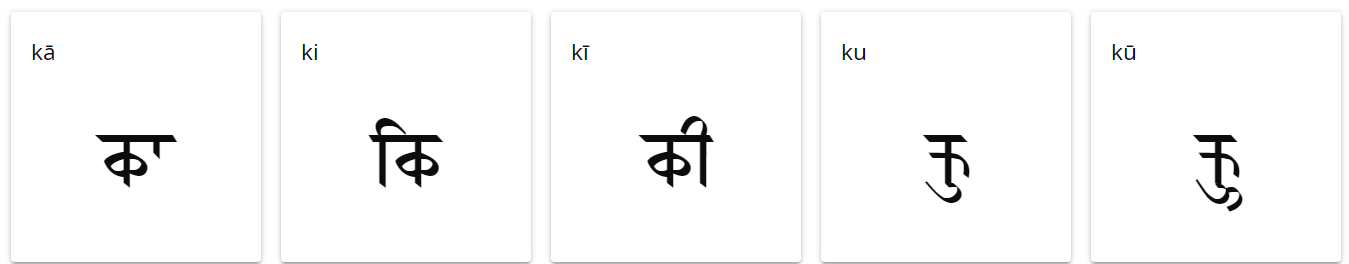
\includegraphics[width=\linewidth,keepaspectratio]{sharada_compounds_kaa} 
	
	{\tiny (Ref: Aksharamukha : Script Converter)}
	\end{center}	

\end{frame}

%%%%%%%%%%%%%%%%%%%%%%%%%%%%%%%%%%%%%%%%%%%%%%%%%%%%%%%%%%%
\begin{frame}[fragile]\frametitle{Compounds}

	\begin{center}
	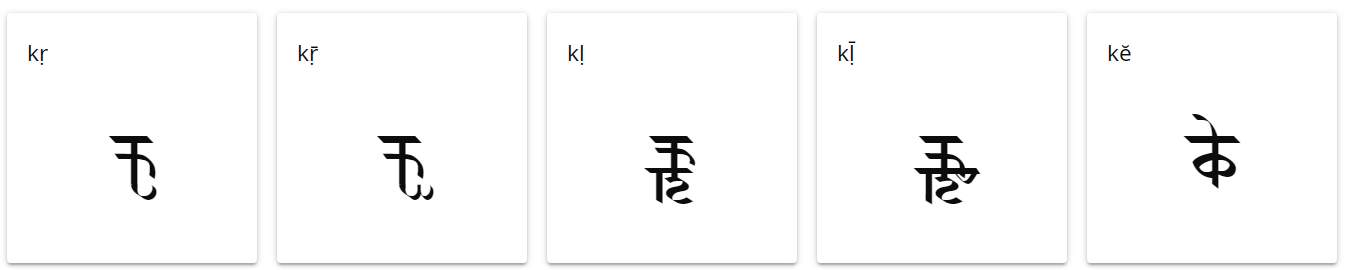
\includegraphics[width=\linewidth,keepaspectratio]{sharada_compounds_kr} 
	
	{\tiny (Ref: Aksharamukha : Script Converter)}
	\end{center}	

\end{frame}

%%%%%%%%%%%%%%%%%%%%%%%%%%%%%%%%%%%%%%%%%%%%%%%%%%%%%%%%%%%
\begin{frame}[fragile]\frametitle{Compounds}

	\begin{center}
	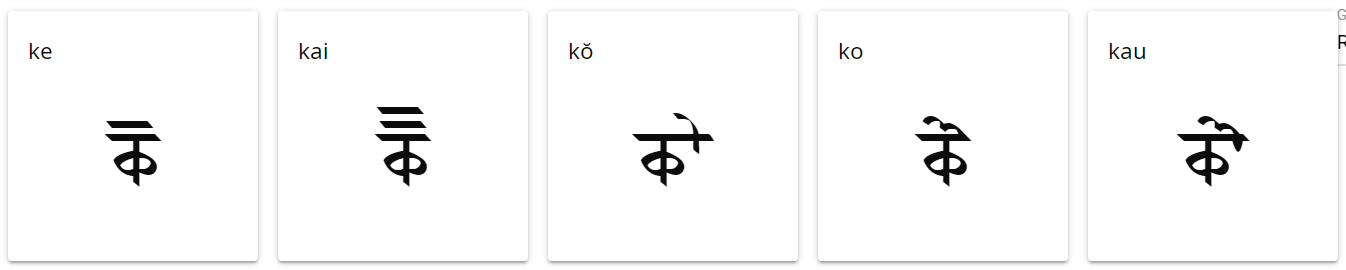
\includegraphics[width=\linewidth,keepaspectratio]{sharada_compounds_ke} 
	
	{\tiny (Ref: Aksharamukha : Script Converter)}
	\end{center}	

\end{frame}

%%%%%%%%%%%%%%%%%%%%%%%%%%%%%%%%%%%%%%%%%%%%%%%%%%%%%%%%%%%
\begin{frame}[fragile]\frametitle{Compounds}

	\begin{center}
	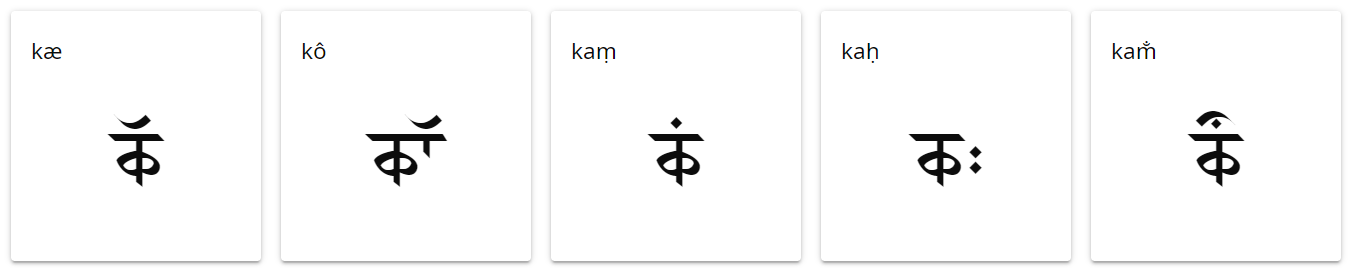
\includegraphics[width=\linewidth,keepaspectratio]{sharada_compounds_kae} 
	
	{\tiny (Ref: Aksharamukha : Script Converter)}
	\end{center}	

\end{frame}

%%%%%%%%%%%%%%%%%%%%%%%%%%%%%%%%%%%%%%%%%%%%%%%%%%%%%%%%%%%
\begin{frame}[fragile]\frametitle{Compounds}

	\begin{center}
	
\includegraphics[width=\linewidth,keepaspectratio]{sharada_compounds_k} 
	
	{\tiny (Ref: Aksharamukha : Script Converter)}
	\end{center}	

\end{frame}

%%%%%%%%%%%%%%%%%%%%%%%%%%%%%%%%%%%%%%%%%%%%%%%%%%%%%%%%%%%
\begin{frame}[fragile]\frametitle{Compounds}

	\begin{center}
	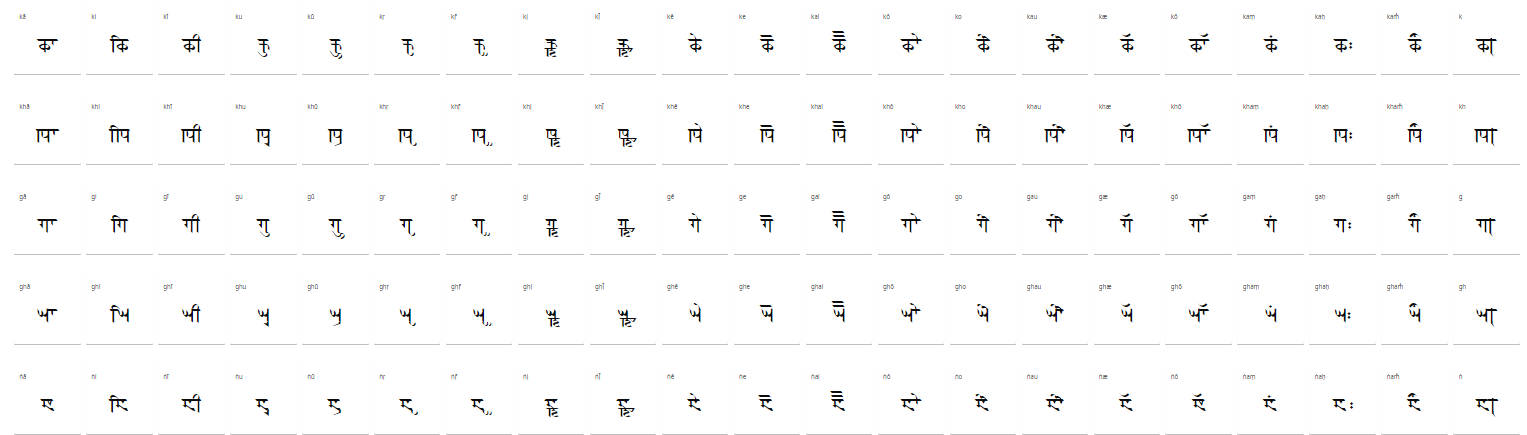
\includegraphics[width=\linewidth,keepaspectratio]{sharada_compounds_ka_varga} 
	
	{\tiny (Ref: Aksharamukha : Script Converter)}
	\end{center}	

\end{frame}

%%%%%%%%%%%%%%%%%%%%%%%%%%%%%%%%%%%%%%%%%%%%%%%%%%%%%%%%%%%
\begin{frame}[fragile]\frametitle{Compounds}

	\begin{center}
	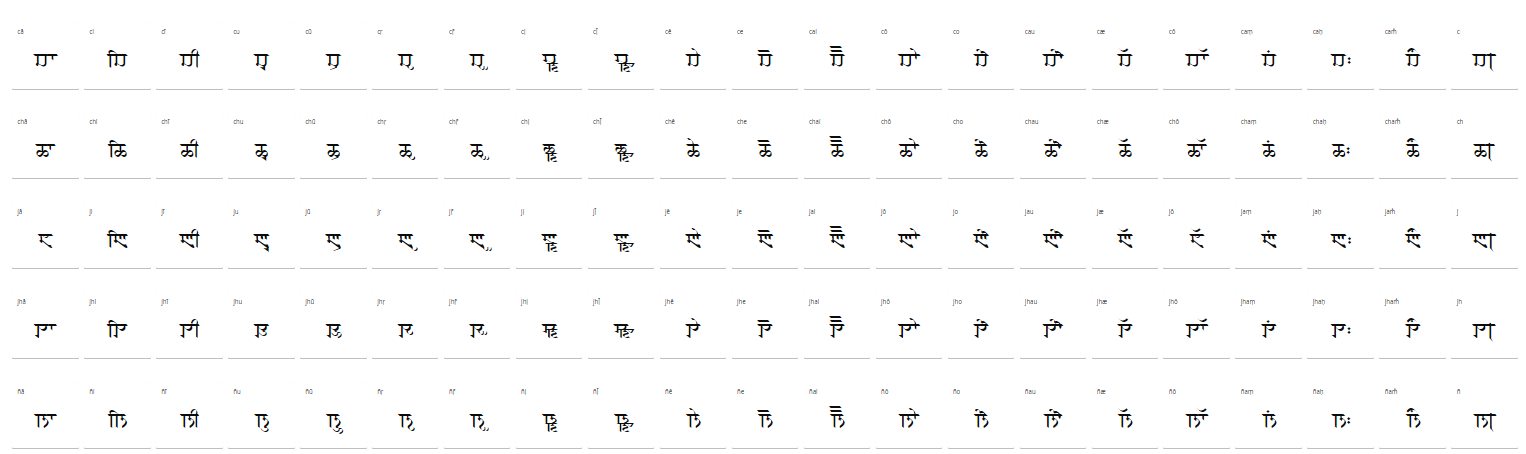
\includegraphics[width=\linewidth,keepaspectratio]{sharada_compounds_cha_varga} 
	
	{\tiny (Ref: Aksharamukha : Script Converter)}
	\end{center}	

\end{frame}

%%%%%%%%%%%%%%%%%%%%%%%%%%%%%%%%%%%%%%%%%%%%%%%%%%%%%%%%%%%
\begin{frame}[fragile]\frametitle{Compounds}

	\begin{center}
	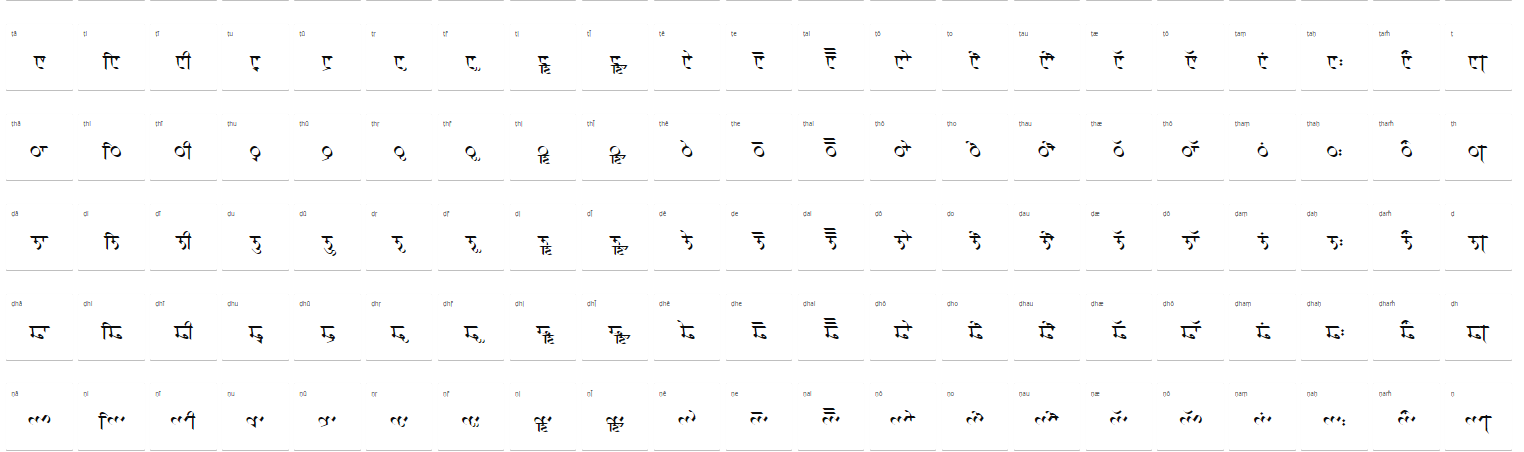
\includegraphics[width=\linewidth,keepaspectratio]{sharada_compounds_Ta_varga} 
	
	{\tiny (Ref: Aksharamukha : Script Converter)}
	\end{center}	

\end{frame}

%%%%%%%%%%%%%%%%%%%%%%%%%%%%%%%%%%%%%%%%%%%%%%%%%%%%%%%%%%%
\begin{frame}[fragile]\frametitle{Compounds}

	\begin{center}
	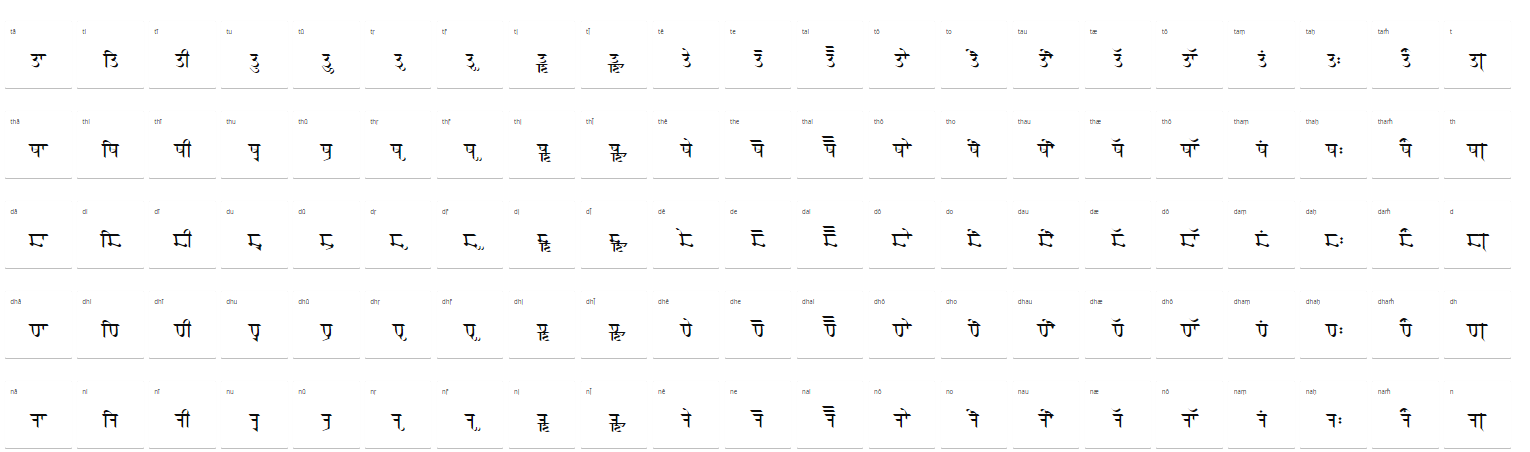
\includegraphics[width=\linewidth,keepaspectratio]{sharada_compounds_taa_varga} 
	
	{\tiny (Ref: Aksharamukha : Script Converter)}
	\end{center}	

\end{frame}

%%%%%%%%%%%%%%%%%%%%%%%%%%%%%%%%%%%%%%%%%%%%%%%%%%%%%%%%%%%
\begin{frame}[fragile]\frametitle{Compounds}

	\begin{center}
	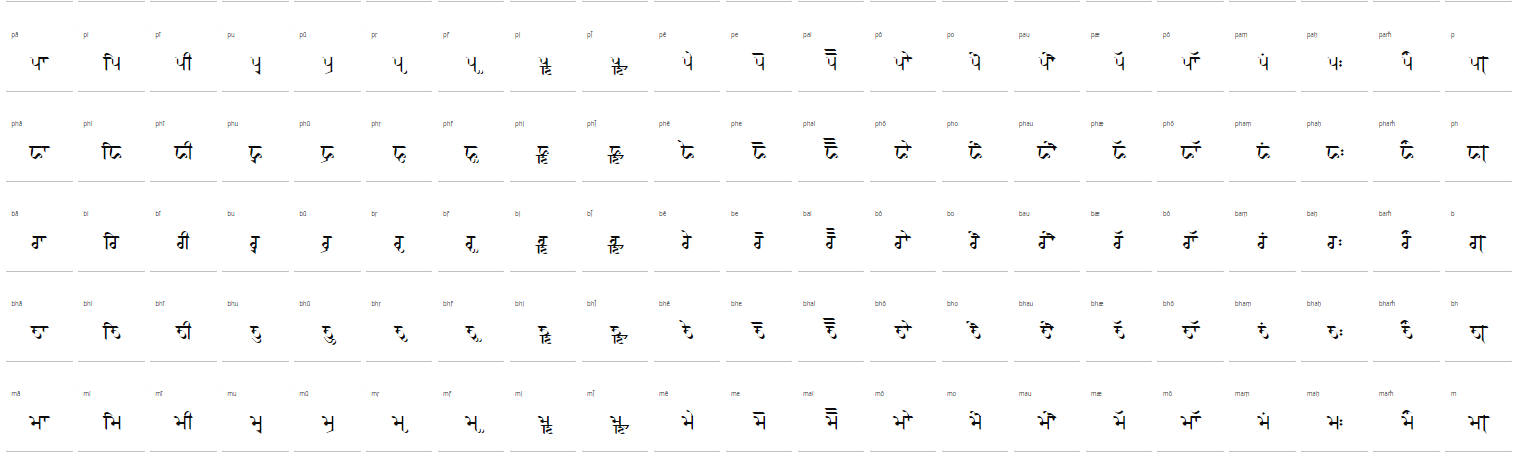
\includegraphics[width=\linewidth,keepaspectratio]{sharada_compounds_pa_varga} 
	
	{\tiny (Ref: Aksharamukha : Script Converter)}
	\end{center}	

\end{frame}

%%%%%%%%%%%%%%%%%%%%%%%%%%%%%%%%%%%%%%%%%%%%%%%%%%%%%%%%%%%
\begin{frame}[fragile]\frametitle{Compounds}

	\begin{center}
	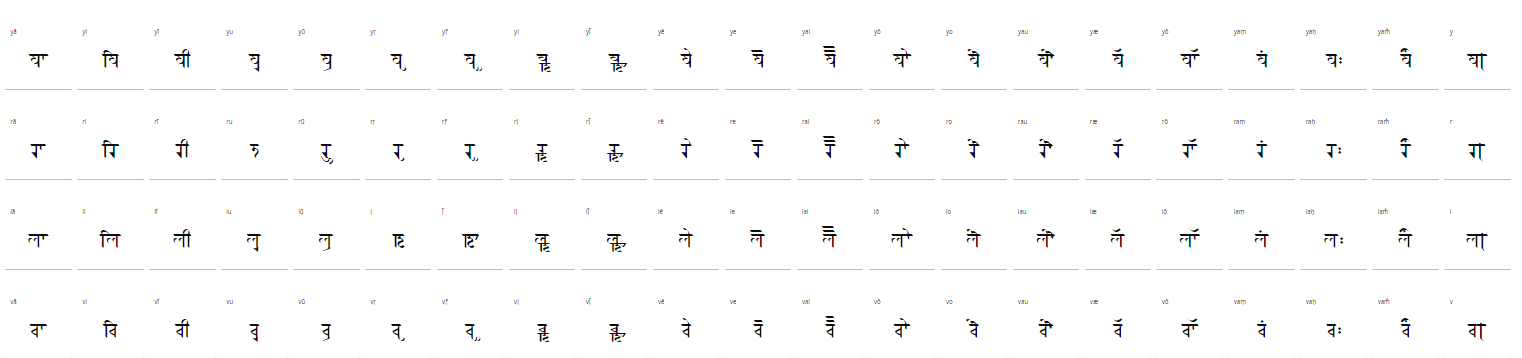
\includegraphics[width=\linewidth,keepaspectratio]{sharada_compounds_ya_varga} 
	
	{\tiny (Ref: Aksharamukha : Script Converter)}
	\end{center}	

\end{frame}

%%%%%%%%%%%%%%%%%%%%%%%%%%%%%%%%%%%%%%%%%%%%%%%%%%%%%%%%%%%
\begin{frame}[fragile]\frametitle{Compounds}

	\begin{center}
	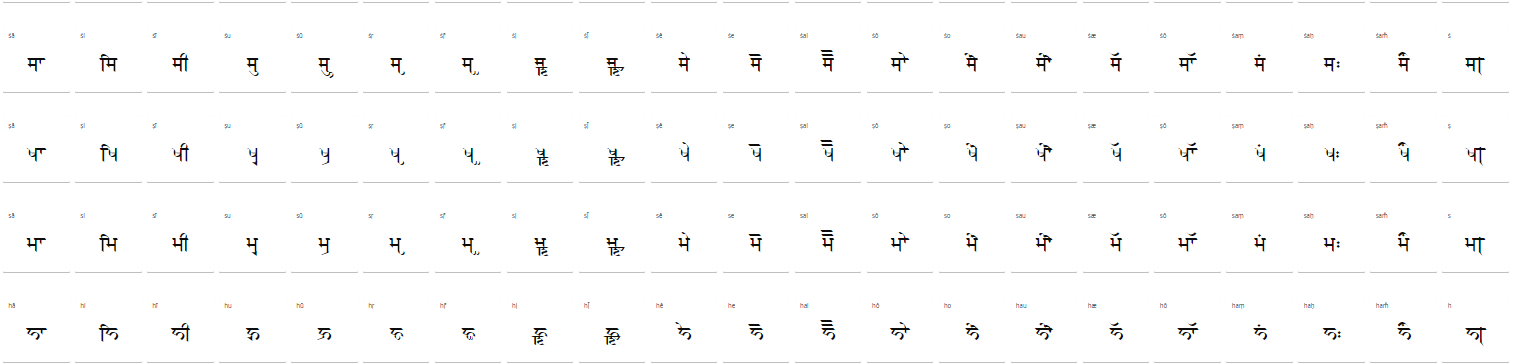
\includegraphics[width=\linewidth,keepaspectratio]{sharada_compounds_sa_varga} 
	
	{\tiny (Ref: Aksharamukha : Script Converter)}
	\end{center}	

\end{frame}

%%%%%%%%%%%%%%%%%%%%%%%%%%%%%%%%%%%%%%%%%%%%%%%%%%%%%%%%%%%
\begin{frame}[fragile]\frametitle{Compounds}

	\begin{center}
	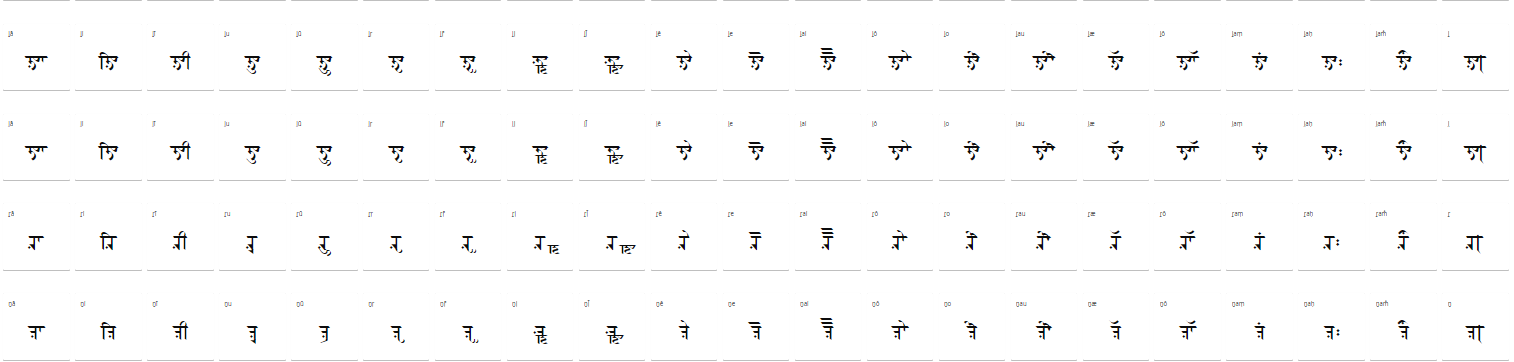
\includegraphics[width=\linewidth,keepaspectratio]{sharada_compounds_la_varga} 
	
	{\tiny (Ref: Aksharamukha : Script Converter)}
	\end{center}	

\end{frame}

%%%%%%%%%%%%%%%%%%%%%%%%%%%%%%%%%%%%%%%%%%%%%%%%%%%%%%%%%%%
\begin{frame}[fragile]\frametitle{Compounds}

	\begin{center}
	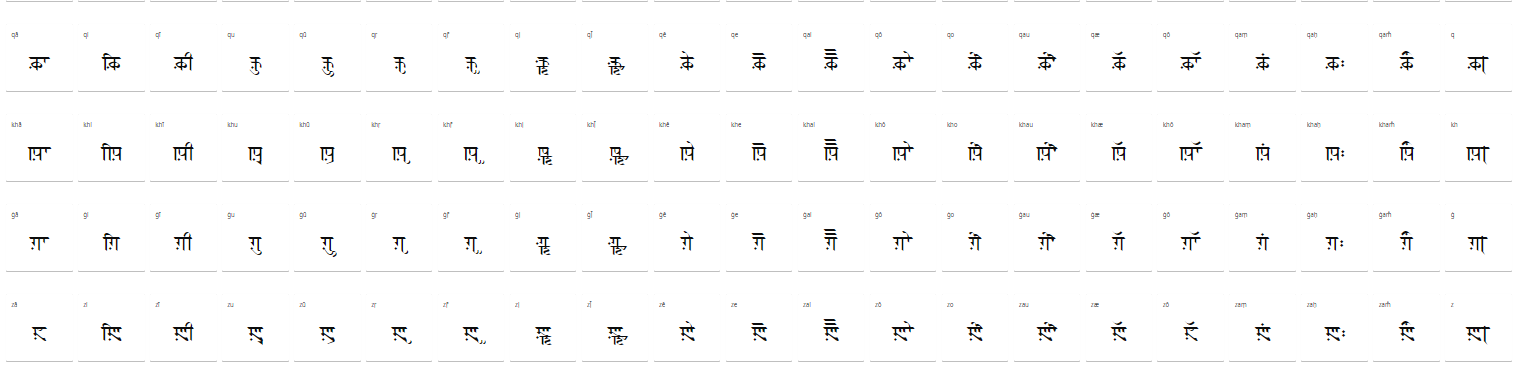
\includegraphics[width=\linewidth,keepaspectratio]{sharada_compounds_qa_varga} 
	
	{\tiny (Ref: Aksharamukha : Script Converter)}
	\end{center}	

\end{frame}

%%%%%%%%%%%%%%%%%%%%%%%%%%%%%%%%%%%%%%%%%%%%%%%%%%%%%%%%%%%
\begin{frame}[fragile]\frametitle{Compounds}

	\begin{center}
	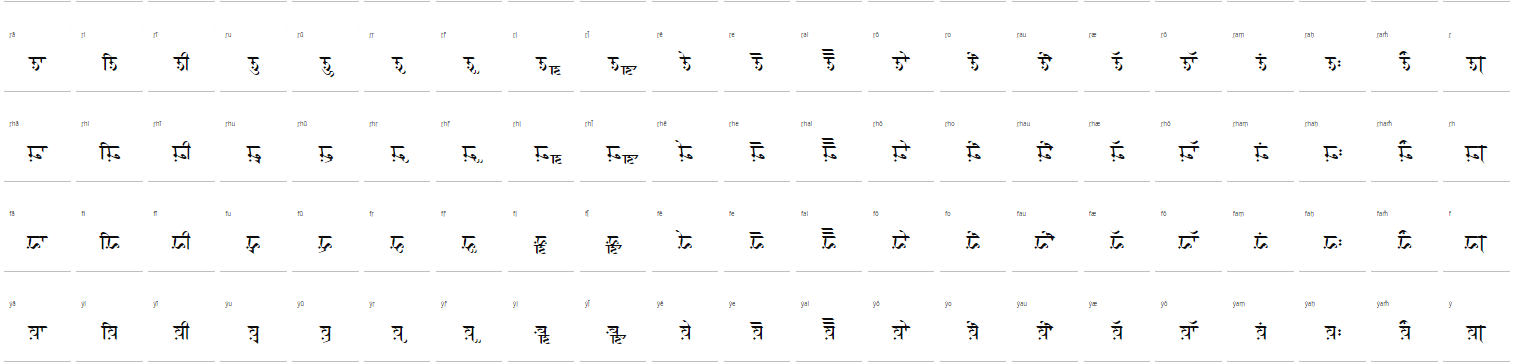
\includegraphics[width=\linewidth,keepaspectratio]{sharada_compounds_ra_varga} 
	
	{\tiny (Ref: Aksharamukha : Script Converter)}
	\end{center}	

\end{frame}

\section[Trans]{Transliteration}
%%%%%%%%%%%%%%%%%%%%%%%%%%%%%%%%%%%%%%%%%%%%%%%%%%%%%%%%%%%%%%%%%%%%%%%%%%%%%%%%%%
\begin{frame}[fragile]\frametitle{}
\begin{center}
{\Large Transliteration}
\end{center}
\end{frame}


%%%%%%%%%%%%%%%%%%%%%%%%%%%%%%%%%%%%%%%%%%%%%%%%%%%%%%%%%%%
\begin{frame}[fragile]\frametitle{Aksharamukha : Script Converter}


	\begin{lstlisting}
pip install aksharamukha

from aksharamukha import transliterate
transliterate.process(src, tgt, txt, nativize = True, pre_options = [], post_options = [])
transliterate.process('HK', 'Telugu', 'buddhaH')

# If the source script is not known, set it as autodetect
transliterate.process('autodetect', 'IAST', '....')

# You can also convert files (.docx, .html & .txt) as shown below.
from aksharamukha import transliterate_file
transliterate_file.process(src, tgt, file_path, nativize=True, pre_options = [], post_options = [])


# REST API
http://aksharamukha-plugin.appspot.com/
api/public?source=HK&target=Telugu&text=buddhaH
\end{lstlisting}

\end{frame}




\section[End]{Towards End}
%%%%%%%%%%%%%%%%%%%%%%%%%%%%%%%%%%%%%%%%%%%%%%%%%%%%%%%%%%%%%%%%%%%%%%%%%%%%%%%%%%
\begin{frame}[fragile]\frametitle{}
\begin{center}
{\Large References}
\end{center}
\end{frame}


%%%%%%%%%%%%%%%%%%%%%%%%%%%%%%%%%%%%%%%%%%%%%%%%%%%%%%%%%%%
\begin{frame}[fragile]\frametitle{References}

Many publicly available sources have been used in the preparation of this content. Some of the salient ones are listed below:

	\begin{itemize}
	\item Core Sharada Team https://www.shardalipi.com/ Courses, Resources
	\item Learn Sharada Lipi - Learn Sanskrit Online : vyoma-samskrta-pathasala YouTube % https://www.youtube.com/playlist?list=PLmozlYyYE-ETiEDyzg3UYg4pbNz31nCEG
	\item Virtual Vinodh http://www.virtualvinodh.com/projects Transliteration code Github
	\item Satisar https://satisarsharada.appspot.com/editor Online Transliteration App
	\item Sharada script translation - Kashmiri Youth Movement https://kashmiriyouthmovement.org/sharada-script-translation/
	\item Sarada script | South Indian, Tamil-Brahmi, Grantha | Britannica https://www.britannica.com/topic/Sarada-script
	\item Kashmiri transliteration - Wikipedia https://en.m.wikipedia.org/wiki/Kashmiri\_transliteration
	\item Noto Sans Sharada - Google Fonts https://fonts.google.com/noto/specimen/Noto+Sans+Sharada
	\item Shaarda - Sunil M YouTube %https://www.youtube.com/playlist?list=PLkTrUAJaxE7A\_OYBGu2hAXvuMkwZ\_JYWe
	\end{itemize}

\end{frame}


%%%%%%%%%%%%%%%%%%%%%%%%%%%%%%%%%%%%%%%%%%%%%%%%%%%%%%%%%%%
\begin{frame}[fragile]\frametitle{}

\begin{center}
\includegraphics[width=0.8\linewidth,keepaspectratio]{my_yog_back}

Thanks धन्यवाद
\end{center}

\end{frame}

\end{multicols}

\rule{\linewidth}{0.25pt}
\scriptsize
Copyleft \textcopyleft\  Send suggestions to 
\href{http://www.yogeshkulkarni.com}{yogeshkulkarni@yahoo.com}

\end{document}
